\section{Workload Characterization}
\label{sec:workloadchar}
a

Comparing the trends observed in Spider I vs Spider II

\subsection{I/O Usage Trends}
\subsubsection{Atlas1 and Atlas2 Utilization}
-- Bandwidth
-- Controller usage trends

\subsubsection{Read vs Write}
For both Spider I and Spider II

\begin{figure}[!t]
\centering
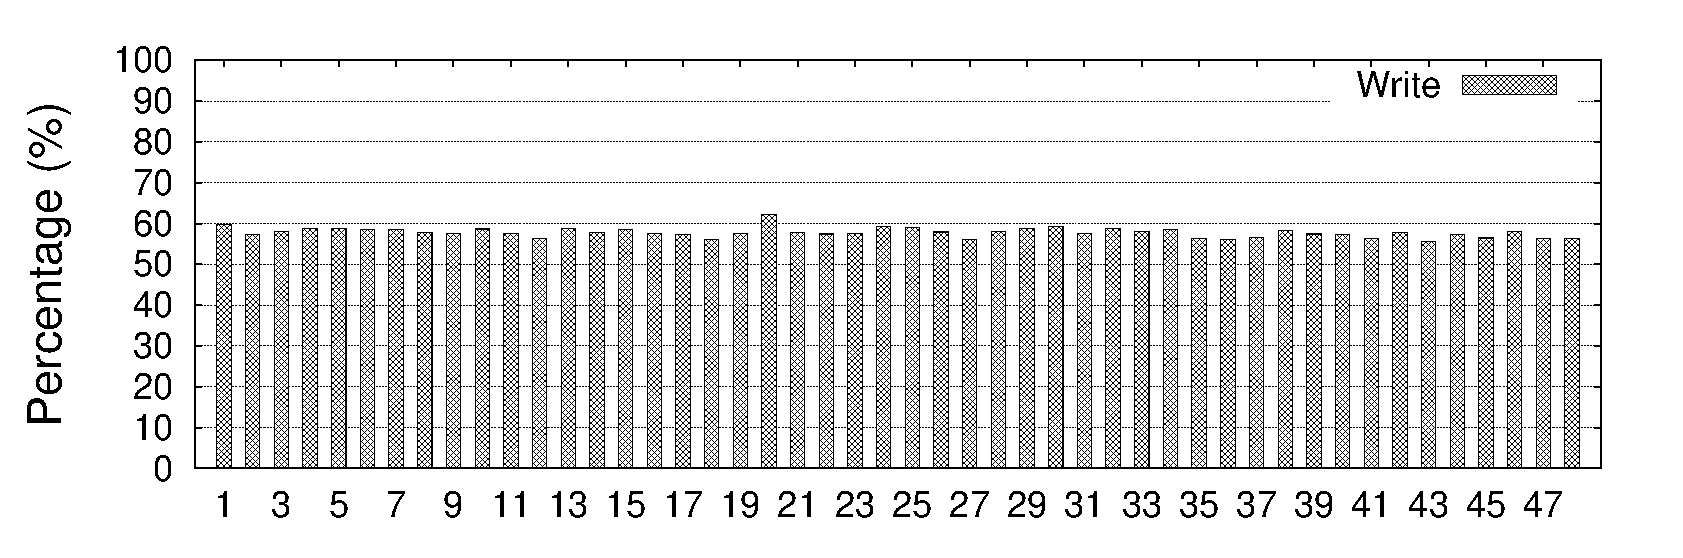
\includegraphics[width=0.5\textwidth]{./figs/spider1-rd-wr-ratio.eps}
%\includegraphics[width=0.5\textwidth]{}
\vspace{-0.1in}
\centering
\caption{Spider - Read Write Ratio}
\label{fig:rwratio}
\end{figure}


\subsection{I/O Requests}
\subsubsection{Request Size distribution}

\begin{figure}[!t]
\begin{center}
\begin{tabular}{cc}
\hspace*{-1cm}                                                           
{\includegraphics[width=0.27\textwidth]{./figs/spider1-reqSizeCDF.eps}}&
\hspace{-2mm}
{\includegraphics[width=0.27\textwidth]{./figs/spider1-reqSizePDF.eps}}\\
\small (a) CDF & \small(b) PDF \\
\end{tabular}
\vspace{-0.1in}
\captionsetup{justification=centering}
\caption{Spider 1 - Distribution of Request Sizes}
\label{fig:spider1-reqsizedist}
\end{center}
\end{figure}

\begin{figure}[!t]
\begin{center}
\begin{tabular}{cc}
\hspace*{-1cm}                                                           
{\includegraphics[width=0.27\textwidth]{./figs/spider2-reqSizeCDF.eps}}&
\hspace{-2mm}
{\includegraphics[width=0.27\textwidth]{./figs/spider2-reqSizePDF.eps}}\\
\small (a) CDF & \small(b) PDF \\
\end{tabular}
\vspace{-0.1in}
\caption{Spider 2 - Distribution of Request Sizes}
\label{fig:spider2-reqsizedist}
\end{center}
\end{figure}

Figure~\ref{fig:spider1-reqsizedist} and Figure~\ref{fig:spider2-reqsizedist} shows
the distribution of read and writes requests on Spider 1
and Spider 2, respectively. The Lustre file system supports a range of request
block sizes, the smallest being 4 kiloBytes (kB) and the largest being 4
MegaBytes (MB).  However, on Spider 1, the smallest block size we were able to
monitor was 16KB, a limitation of the DDN RAID controller. Interpreting from
the CDF and PDF plots here are some interesting observation.

\begin{itemize}

\item  60\% of write requests on Spider 2 where 4kB or less.  In Spider 1, we
unable to distinguish between the 4kB, 8kB and 16kB, which accounted for 50\% of
the write requests.
\item  Also, Spider 2 has 70\% of the requests which are less than or equal to
512kB, whereas on Spider 1, only 55\% of the requests were less than 512kB. ?  
\item   Large number of 512kB requests (SRP ) ?
\item On Spider 2 over 50\% of reads were 1MB, similar to Spider 1 combined
512kB and 1MB were 50\%. However, only 25\% of writes on Spider 2 are 1MB,
whereas on Spider 1 over 45% of writes where either 512kB or 1MB.

\end{itemize}


\subsubsection{Request Size Latency distribution}

\begin{figure}[!t]
\centering
\begin{tabular}{cc}
{\includegraphics[width=0.24\textwidth]{./figs/spider2-reqLatCDF.eps}}&
{\includegraphics[width=0.24\textwidth]{./figs/spider2-reqLatPDF.eps}}\\
\end{tabular}
\vspace{-0.1in}
\centering
\caption{Spider 2 - Request Service Latency distribution}
\label{fig:spider1-reqLat}
\end{figure}




\subsection{Request Size vs Bandwidth}

 
